\documentclass{report}


\usepackage[catalan]{babel}
% Instrucci� a Windows per a que accepti els caracters amb accents (� � � � �...)
\usepackage[ansinew]{inputenc}
% Instrucci� a Unix per a que accepti els caracters amb accents (� � � � �...)
% \usepackage[latin1]{inputenc}

% Opcions a usar per PostScript
\usepackage[dvips] {graphicx}
\usepackage[dvips] {color}
%\input{epsf}
\usepackage{epsfig}
% Opcions a usar per PDF
%\usepackage[pdflatex] {graphicx}

%Pel simbol del euro
\usepackage{eurosym}

%Per poder fer multirow als tabulars
\usepackage{multirow}

%Para javadoc---------
\usepackage{amsfonts}
\usepackage{amsmath}
\usepackage{ifthen}
\definecolor{Light}{gray}{.90}
%---------------------

\linespread{1.5}

\definecolor{gris}{gray}{0.9}



\setcounter{secnumdepth}{3} \setcounter{tocdepth}{3}
\author{Java-KLASS versi� 6}
\title{Manual d'instal�laci�}




\begin{document}
\setlength{\baselineskip}{1.5em}
\setlength{\parskip}{0em}
\setlength{\parsep}{0.5em}
\newfont{\peq}{cmbx9}

% Definici� del estil pels exemples,...
\newenvironment{exemple}{\begin{quote}\small {\bf Exemple:}}{\end{quote}}
% Definici� entorn demo
\newcommand{\cuadradito}{\vrule width 1.4mm height 1.4mm depth 0 mm}
\newcommand{\qed}{\hbox{}\nobreak \hfill \cuadradito \par \goodbreak \smallskip}
\newenvironment{demo}{\begin{quote}\small {\bf Demostraci�}} {\qed \end{quote}}
% Definici� Descripci�
\newcommand{\descrip}{\indent{\large \sffamily Descripci�}}
% Definici� Atributs
\newcommand{\atrib}{{\indent\large \sffamily Atributs}}
% Definici� M�todes
\newcommand{\metod}{{\indent\large \sffamily Operacions}}

% Per posar la l geminada (encara que existeix una altra manera: \l.l)
\newcommand{\lge}[1]{\hbox{#1\kern-.1em\raise.5ex\hbox{.}\kern-.1em #1}}
\alph{enumii}\roman{enumii}

%%%%%%%%%%%%emieza titulo


\maketitle




%%%%%%%%%%%%%%%%%%termina tutuolo

%%%% inici texte
%\input{portadaTIT.tex}
%\input{agrair.tex}
% Index general
\tableofcontents
% Index de figures
%\listoffigures
% Index de taules
%\listoftables
%\input{capitulo1/intro.tex}
%\input{capitol2/conceptes.tex}
%\input{capitol3/basesConeixement.tex}
%\input{capitol4/requeriments.tex}
%\input{capitol5/estructures.tex}
%\input{capitol6/especificacio.tex}
%\input{capitol7/disseny.tex}
%\input{capitol8/implementacio.tex}
%\input{capitol9/cost.tex}
%\input{capitol10/conclusions.tex}
% \addcontentsline{toc}{chapter}{Bibliografia}
%\bibliographystyle{alpha}

% \bibliography{bibliografia/biblio1,bibliografia/marbib,bibliografia/biblio2}

% Afegim les cites que encara que no s'hagin referenciat interessa que surtin
%\nocite{*}

% ANNEXOS
%\appendix
%\input{instalacio/manualInstal.tex}
 %\chapter{Manual d'usuari}
\label{sec:ManualDus}

\newpage

\vspace*{5cm}

\begin{center}


{\Huge\bf JAVA-KLASS v2.0

\vspace*{1cm}

  Manual d'usuari}

\vspace*{2cm}

Jose Ignacio Mateos Clavero

M� del Mar Colillas

Karina Gibert Oliveras

juliol de 2007


\end{center}



 \newpage
En aquest manual es proporcionen algunes explicacions per facilitar
l'�s de l'aplicaci� als nous usuaris.

\section{Tipus de finestres i disseny de formularis a Java-KLASS}

\subsection{Tipus de finestres}

L'aplicaci� \textbf{Java-KLASS} t� b�sicament tres tipus de
finestres:
\begin{itemize}



    \item La \emph{finestra b�sica} (veure figura \ref{fig:Basica}): �s la finestra principal de l'aplicaci�, que sempre estar� oberta mentre l'aplicaci� estigui oberta, i on es van mostrant els formularis principals de les diferents funcionalitats a les que es tenen acc�s. T� tres �rees diferenciades, com es pot veure a les figures \ref{fig:Basica} i \ref{fig:UnivError}:

\begin{figure}[ht]
    \centering
        \includegraphics[width=\textwidth]{usuari/pantalles/Basica.eps}
    \caption{Finestra b�sica: 1)\emph{barra de men�s}; 2)\emph{panell central}; 3)\emph{barra d'estat}}
    \label{fig:Basica}
\end{figure}

        \begin{enumerate}
            \item Barra de men�s: sempre es troba a la part superior de la finestra i permet accedir a les funcionalitats de l'aplicaci�.
            \item Panell central: es troba a la zona central de la finestra i �s on es mostren els formularis que permeten introduir tota la informaci� perqu� es realitzi l'operaci� desitjada. Si no es t� seleccionada cap operaci� aquest panell estar� buit com �s veu a la figura \ref{fig:Basica}.
            \item Barra d'estat: es troba a la part inferior de la finestra i �s la zona on apareixen els missatges d'error o informatius resultants de les operacions que es realitzen a la aplicaci�.
        \end{enumerate}


\begin{figure}[ht]
    \centering
        \includegraphics[width=\textwidth]{usuari/pantalles/UnivError.eps}
    \caption{Estructura de la finestra b�sica}
    \label{fig:UnivError}
\end{figure}


    \item La \emph{finestra d'opcions} (veure figura \ref{fig:OpcHisto} i \ref{fig:OpcMinko}): �s la que permet que es puguin especificar les opcions amb les que vol que es realitzi el c�lcul que s'ha seleccionat. S'hi accedeix mitjan�ant els botons d'Opcions que apareixen als formularis de la finestra b�sica. S'estructura de la seg�ent manera:
        \begin{enumerate}
            \item a la zona superior es mostraran les diferents opcions que pot seleccionar l'usuari pel c�lcul o gr�fic seleccionat.
            \item a la part inferior tindr� tres botons per tornar a les opcions per defecte establertes pel sistema, per guardar les modificacions introdu�des i per cance\lge lar l'operaci� de modificaci� de les opcions; el bot� de les opcions per defecte s'ha separat per distingir aquesta funcionalitat de la resta.
        \end{enumerate}



\begin{figure}[ht]
    \centering
        \includegraphics[width=\textwidth]{usuari/pantalles/OpcHisto.eps}
    \caption{Finestra d'opcions 1}
    \label{fig:OpcHisto}
\end{figure}

\begin{figure}[ht]
    \centering
        \includegraphics[width=0.5\textwidth] {usuari/pantalles/min.eps}
    \caption{Finestra d'opcions 2}
    \label{fig:OpcMinko}
\end{figure}



    \item La \emph{finestra de confirmaci�} (veure figura \ref{fig:ConfirmarDef}): �s la que apareix per demanar que es confirmi una acci� abans que el sistema la dugui a terme. Aix�, es mostrar� a la part superior un pregunta, que s'haur� de contestar polsant un dels botons de la part inferior.

\newpage

\end{itemize}
\begin{figure}[ht]
    \centering
        
\includegraphics[width=\textwidth]{usuari/pantalles/ConfirmarDef.eps}
    \caption{Finestra de confirmaci�}
    \label{fig:ConfirmarDef}
\end{figure}



\subsection{Disseny de formularis}

El disseny de formularis de \textbf{Java-KLASS} va seguint sempre la
mateixa filosofia i s'ha intentat que siguin el m�s homog�nies
possible, fent que a tots apareguin els seg�ents elements, amb
variacions depenent de les necessitats de cada cas:
\begin{itemize}
    \item Llista de variables que conformen la matriu de dades, diferenciant les num�riques de les categ�riques.
    \item Llista de variables seleccionades sobre les que realitzar les diferents operacions, de forma que es pugui realitzar una mateixa combinaci� de c�l\-culs i gr�fics per diverses variables (o parells o ternes) alhora. Aquesta pos\-si\-bi\-li\-tat pro\-por\-cio\-na molta pot�ncia al sistema i permet que, amb una sola es\-pe\-ci\-fi\-ca\-ci�, s'analitzi tot el joc de dades.
    \item Botons per poder passar elements de la llista general de variables a la llista de seleccionades, i a l'inrev�s. Aix� proporciona comoditat, doncs permet, per exemple, seleccionar o eliminar totes les variables de cop.
    \item Selecci� m�ltiple de c�lculs o representacions gr�fiques a realitzar amb les variables seleccionades, diferenciant tamb� unes de les altres segons el tipus de variable o combinaci� de variables sobre les que s'apliquen.
    \item Bot� d''Opcions' al costat de cada c�lcul o gr�fic que permet indicar diferents modificacions que s'expliquen m�s endavant. Aquest bot� nom�s estar� habilitat quan el c�lcul o gr�fic corresponent estigui seleccionat.
    \item Bot� 'Per defecte' que permet passar a seleccionar la configuraci� mes adient per a les dades carregades. Com s'ha comentat en la introducci� sobre les finestres d'opcions, aquest bot� s'ha separat dels altres per q�estions d'usabilitat, per facilitar a l'usuari la distinci� d'aquesta funcionalitat de la resta.
    \item Bot� 'D'acord' per passar a executar la petici� de c�lcul;
    \item Bot� 'Cance\lge lar' per suspendre la petici� demanada.
    \item Bot� 'Netejar' elimina tota la selecci� d'opcions i dades
    introdu�des per deixar el formulari \emph{net}.
\end{itemize}


\begin{figure}[ht]
    \centering
        \includegraphics[width=\textwidth]{usuari/pantalles/Biv.eps}
        \caption{Menu Descriptiva Bivariant}
        \label{bivari}
\end{figure}

\newpage

Pel que fa a la distribuci� d'aquest elements a la pantalla, cal
remarcar que atenent al fet que alguns gr�fics o c�lculs requereixen
variables de tipus espec�fics es presenten en llistes separades els
grups de variables seleccionades segons es combinen els seus tipus
,per exemple, \textit{num $\times$ num}, o \textit{cat $\times$ cat
$\times$ num} del formulari d'estad�stica descriptiva bivariant de
la fig \ref{bivari}. En tot moment s'ha buscat la proximitat f�sica
entre la llista d'on triar les variables i la de selecci�. A m�s, al
costat o sota de cada llista, depenent de la disposici� de la
finestra, es presenten els c�lculs o gr�fics corresponents a aquella
combinaci�. En general, s'ha buscat que el formulari quedi dividit
en �rees i que les diferents c�lculs o gr�fics quedin f�sicament a
prop de les variables seleccionades.



\section{Funcionalitats de Java-KLASS}

\subsection{Menu principal}

La barra de men�s de la finestra b�sica s'ha organitzat en nou
submen�s desplegables que es cor\-res\-po\-nen amb els grups de
funcionalitats definits a l'aplicaci�. La part de gesti� de dades
s'ha dividit en dos per distingir les funcionalitats de gesti� de
dades que impliquen expl�citament la lectura o escriptura de fitxers
seguint l'est�ndard Windows. Hi ha moltes de les funcionalitats que
es troben en desenvolupament o encara no s'han asigant a cap
desenvolupador, i encara que les anomenarem no podran ser
seleccionades per l'usuari. D'acord amb aix�, els submen�s queden
estructurats seguint la seg�ent jerarquia:
\begin{itemize}
    \item \emph{Fitxer}
        \begin{itemize}
            \item \emph{Obre}: Permet carregar diferents arxius.
            \begin{itemize}
                \item \emph{Dades sense regles}: Permet carregar una matriu de dades sense regles a partir de fitxers en format KLASS (explicat a l'ap�ndix \ref{fitxers entrada}),actualment {\bf Java-KLASS v2.0} permet fins a 10 matrius obertes simultaneament.
                \item \emph{Dades amb regles}: Permet carregar una matriu de dades amb regles.
                \item \emph{Regles}: Aquesta opci� nom�s est� activa si en el sistema hi ha alguna matriu de dades carregada i serveix per importar una base de coneixement en format de fitxer .reg
                \item \emph{Dendograma}: Aquesta opci� nom�s est�
                activa si en el sistema hi ha alguna matriu de dades carregada i serveix per importar una classificaci� ascendent
            jer�rquica de la matriu activa a partir d'un fitxer nomMatriuActiva.drm.
                \item \emph{Hist�ria}: Aquesta opci� nom�s est� activa si en el sistema hi ha alguna
matriu de dades carregada i serveix per importar una classifcaci�
ascendent jer�rquica de la matriu activa a partir d'un fitxer
nomMatriuActiva.his.
            \end{itemize}
            \item \emph{Tanca}: Permet tancar la matriu actual amb la que s'est� treballant, deixant de tenir-la carregada al sistema.
            \item \emph{Anomena i desa}: Salva la matriu actual amb la que s'est� treballant en format KLASS.
            \item \emph{Importa}: Permet importar una matriu de dades en format .dat est�ndard.
            \item \emph{Exporta}: Permet exportar una matriu de dades en format .dat est�ndard.
            \item \emph{Configuraci�}: Permet configurar el nombre m�xim de matrius car\-re\-ga\-des al sistema, i les comandes que l'aplicaci� far� servir per compilar els fitxers font de {\LaTeX} i generar DVI o PDF, i tamb� les comandes per visualitzar-los.
            \item \emph{Localitzaci� de resultats}: Permet seleccionar quin sera el directori dest� dels fitxers de resultat.
            \item \emph{Surt}: Permet sortir de l'aplicaci� tancant totes les matrius carregades al sistema.
        \end{itemize}
    \item \emph{Dades}
        \begin{itemize}
        \item \emph{Seleccionar submatriu}: Permet crear una nova matriu de dades per selecci� de columnes (variables) i de files (objectes) de la matriu actual.
        \item \emph{Tractament de mancants}: Permet subtituir tots els missings de la matriu per un valor.
        \item \emph{Integra classificaci�}: Afegeix a la matriu de dades en curs una columna nova que cont� la classe de pertinen�a de cada
                                                    objecte, llegint un fitxer d'extensi� \emph{.cls}.
        \item \emph{Canvia matriu actual}: Permet canviar la matriu activa amb la que treballa l'aplicaci�.
        \item \emph{Defineix ordenacions}: Permet definir l'ordre amb que es presentar�n les variables de la matriu activa \emph {(i les modalitats de cada variable categ�rica)} en els informes de resultats de \textbf{Java-KLASS}.
         \item \emph{Matriu de dades}: Mostra una taula que visualitza la matriu actual.
      \end{itemize}
    \item \emph{Descriptiva}
        \begin{itemize}
            \item \emph{Univariant}: Permet realitzar l'an�lisi descriptiva univariant d'una o m�s variables seleccionant els elements descriptius univariants (gr�fics i num�rics) a mostrar.
            \item \emph{Bivariant}: Permet realitzar l'an�lisi descriptiva bivariant d'un o m�s parells de variables seleccionant els elements descriptius bivariants (gr�fics i num�rics) a mostrar en cada cas.
            \item \emph{Matriu de correlacions/covari�ncies}: Permet calcular la matriu de correlacions o covari�ncies d'un conjunt de variables num�riques.
            \item \emph{Trivariant}: Permet realitzar l'an�lisi descriptiva trivariant d'una o m�s ternes de variables seleccionant els elements descriptius trivariants (gr�fics i num�rics) a mostrar en cada cas.
            \item \emph{Descr. per classes}: Permet realitzar l'an�lisi descriptiva d'una o m�s  variables seleccionant els elements descriptius (gr�fics i num�rics) a mostrar en cada cas,
            segons les classes que indiqui la variable de classe.
        \end{itemize}
    \item \emph{Classificaci�}
        \begin{itemize}
            \item \emph{Classifica}: Realitza una classificaci� autom�tica de la matriu de dades per diferents metodes.
            \item \emph{Dendograma}: Aquesta opci� nom�s est� activa
            si en el sistema hi ha alguna classificaci� ascendent
            jer�rquica de la matriu activa, ja sigui perqu� s'ha
            realitzat dins el propi sistema o perqu� s'ha importat
            d'un altre entorn. Si existeixen classificacions es
            podr�n realitzar les seg�ents operacions:
            \begin{itemize}
                \item \emph{Visualitza}: Representa gr�ficament
                l'arbre ascendent jer�rquic.
                \item \emph{Talla arbre}: Permet practicar talls
                horitzontals de l'arbre segons diferents criteris.
                \item \emph{Produeix classificaci�}: Nom�s activa si
                s'han realitzat talls en alg�n arbre del sistema. En
                aquest cas genera  una columna amb la classe de
                pertinen�a de cada objecte de la matriu de dades
                segons el tall seleccionat i permet generar un
                fitxer de format .cls.
            \end{itemize}
        \end{itemize}
    \item \emph{Dist�ncies}
        \begin{itemize}
            \item \emph{C�lcul Directe}: Permet calcular diferents dist�ncies entre 2 vectors introdu�ts per l'usuari.
            \item \emph{C�lcul Matriu}: Permet calcular les diferents dist�ncies sobre la matriu de dades activa.
        \end{itemize}
    \item \emph{Interpretaci�}
        \begin{itemize}
            \item \emph{Discretitzaci� "boxplot-based"}: A partir
            d'una variable de classe, discretitza una variable
            num�rica pel m�tode \emph{boxplot-based
            discretitzation.}
        \end{itemize}
    \item \emph{Informes}
        \begin{itemize}
            \item \emph{Informe autom�tic}: Permet generar un informe autom�tic sobre la matriu actual.
            \item \emph{Informe personalitzat}: Permet generar un
            informe amb el contingut que dissenyi l'usuari.
            \item \emph{Visualitzar Latex}: Permet seleccionar
            fitxers latex ja creats per l'aplicaci� per tornar-los a
            visualitzar.
        \end{itemize}
    \item \emph{S�te\lge lits}
        \begin{itemize}
            \item \emph{CIADEC}: Permet accedir al s�te\lge lit CIADEC.
            \item \emph{Columbus}: Permet accedir al s�te\lge lit Columbus.
        \end{itemize}
    \item Ajuda:
        \begin{itemize}
            \item \emph{Manual}: Visualitza aquest manual en pantalla.
            \item \emph{Quant al Java-KLASS}: Permet accedir a la informaci� sobre \textbf{Java-KLASS}.
        \end{itemize}
\end{itemize}


\subsection{Fitxer} \label{Fitxer}
L'opci� Fitxer, permet tant obrir com guardar matrius de dades i
altres estructures que es manipulen dins l'aplicatiu.

\subsubsection{Obre}
Aquesta opci� �s la que permet carregar les matrius de dades dintre
del sistema, hi ha diferents matrius a carregar i per cada una
s'utilitza un del submen�s seg�ents:

\paragraph{Dades sense Regles} Permet carregar l'estructura b�sica de {\bf Java-KLASS} que �s una matriu de dades
a partir de fitxers en format {\bf KLASS}, �s a dir la informaci�
per a definir una matriu de {\bf Java-KLASS} est� dividida en
fitxers \emph{.dat .obj i .pro.}.

\begin{figure}[ht]
    \centering
        \includegraphics[width=\textwidth]{usuari/pantalles/senseregles.eps}
    \caption{Dades sense Regles}
    \label{fig:sensereg}
\end{figure}


Al \emph{premer} sobre l'opci� es mostra el directori de lectura de
dades per defecte, �s a dir el subdirectori \emph{dades} de la
carpeta on est� instal�lat {\bf Java-KLASS}, es permet navegar pel
sistema de directoris \emph{(veure figura \ref{finestra})} i
seleccionar la matriu que es vol carregar, despr�s aquesta matriu es
carrega al sistema automaticament i es deixa com a matriu activa,
conservant les que ja estaven obertes com a desactivades.

Al navegar pels diferents subdirectoris, unicament es mostren
aquells fitxers dels que existeix la fam�lia completa \emph{.dat
.obj i .pro.}.


\begin{figure}[ht]
    \centering
        \includegraphics[width=\textwidth]{usuari/pantalles/directo.eps}
    \caption{Finestra del directori de dades}
    \label{finestra}
\end{figure}

\newpage

\paragraph{Dendograma...}

Aquesta opci�, nom�s activa si hi ha una matriu de dades carregada
al sistema, carrega un arxiu \emph{.cls} que conte una columna amb
la classe de pertinen�a de cada objecte de la matriu de dades segons
el tall preseleccionat.

\begin{figure}[ht]
    \centering
        \includegraphics[width=\textwidth]{usuari/pantalles/dendo.eps}
    \caption{Dendograma...}
\end{figure}


\newpage

\subsubsection{Tanca}
Aquesta opci� nom�s estar� activa si primer s'ha caregat alguna
matriu, ja que sino no es podra tancar. Tancar �s l'opci� que
elimina la matriu activa de la llista de matrius carregades al
sistema. Al \emph{premer} sobre l'opci� sortir� un di�leg de
confirmaci� per confirmar que es vol eliminar.

\begin{figure}[ht]
    \centering
        \includegraphics[width=\textwidth]{usuari/pantalles/tanca.eps}
    \caption{Menu Tanca}
\end{figure}

\newpage


\subsubsection{Anomena i desa}
Aquesta opci� permet guardar la matriu activa si primer s'ha caregat alguna matriu.

\begin{figure}[ht]
    \centering
        \includegraphics[width=\textwidth]{usuari/pantalles/anomena.eps}
    \caption{Menu Anomena i desa}
\end{figure}

\newpage

Al \emph{premer} sobre l'opci� apareix una finestra que indica el
directori per defecte on s�n les dades, i un quadre de text per
escriure el nom amb el qual es vol guardar la matriu. Al
\emph{premer} guardar, es guardar� la matriu amb els diferents
.dat,.pro i .obj, la figura \ref{ano} mostra aquesta finestra.

\newpage

\begin{figure}[ht]
    \centering
        \includegraphics[width=\textwidth]{usuari/pantalles/anomena1.eps}
    \caption{Finestra per guardar la matriu}
    \label{ano}
\end{figure}


\subsubsection{Configuraci�}
Per defecte, l'aplicaci� utilitza uns parametres per a la configuraci� del m�xim de matrius carregades i la localitzaci� dels
ejecutables per constru�r i visualitzar els arxius {\LaTeX}.

\newpage

\begin{figure}[ht]
    \centering
        \includegraphics[width=\textwidth]{usuari/pantalles/conf.eps}
    \caption{Menu Configuraci�}
\end{figure}

Al \emph{premer} sobre l'opci� apareix una finestra on es pot
seleccionar la ruta dels ejecutables de {\LaTeX} i canviar el nombre
m�xim de matrius al sistema, la figura \ref{config2} mostra aquesta
finestra.

\newpage


\begin{figure}[ht]
    \centering
        \includegraphics[width=\textwidth]{usuari/pantalles/config.eps}
    \caption{Finestra de Configuraci�}
    \label{config2}
\end{figure}


\subsubsection{Localitzaci� de resultats}
Per defecte, l'aplicaci� genera els resultats en un subdirectori
anomenat \emph{'resultats'} dins del directori on estan els fitxers
de la matriu de dades.

\newpage

\begin{figure}[ht]
    \centering
        \includegraphics[width=\textwidth]{usuari/pantalles/loc.eps}
    \caption{Menu Localitzaci� de resultats}
\end{figure}


Al \emph{premer} sobre l'opci� apareix un di�leg de confirmaci� per
confirmar si es vol canviar la localitzaci� actual dels fitxers
resultats.



\begin{figure}[ht]
     \centering
         \includegraphics[width=0.7\textwidth]{usuari/pantalles/loc3.eps}
     \caption{Finestra de confirmaci�}
\end{figure}


Al indicar que es vol canviar es mostra una finestra amb el men� per
seleccionar qualsevol altre directori on l'aplicaci� guardar� els
fitxers resultats que generi.

\newpage

\begin{figure}[ht]
     \centering
         \includegraphics[width=\textwidth]{usuari/pantalles/loc2.eps}
     \caption{Finestra de directoris per Localitzaci� de resultats}
\end{figure}



\subsubsection{Surt}
Aquesta opci� es la que tanca l'aplicatiu.

\newpage

\begin{figure}[ht]
     \centering
         \includegraphics[width=\textwidth]{usuari/pantalles/surt.eps}
     \caption{Menu Surt}
\end{figure}



\subsection{Dades} \label{Dades}
L'opci� Dades, permet manipular la matriu de dades activa, per
obtenir una nova matriu amb alguns canvis necesaris per fer algun
tipus d'operaci�.


\subsubsection{Selecciona Submatriu}

Dintre del menu \emph{Dades} es troba un formulari per seleccionar
una sub-matriu de la matriu activa.

\newpage

\begin{figure}[ht]
     \centering
         \includegraphics[width=\textwidth]{usuari/pantalles/sel.eps}
     \caption{Menu Selecciona Submatriu}
\end{figure}



Com es pot veure en la figura \ref{fig:Sub} el formulari t� 2 �rees
clares. Esquerra per les variables i dreta pels objectes. Hi ha 3
apartats per omplir.

\begin{itemize}
    \item \emph{Variables Num�riques}: On seleccionem de la llista de les variables num�riques originals, quines volem mantenir a la matriu resultant.
    \item \emph{Variables Categ�riques}: On seleccionem de la llista de les variables categ�riques originals, quines volem mantenir a la matriu resultant.
    \item \emph{Objectes}: On seleccionem de la llista d'objectes originals, quins volem mantenir a la matriu resultant.
\end{itemize}

\newpage

\begin{figure}[ht]
    \centering
       \includegraphics[width=\textwidth]{usuari/pantalles/Sub.eps}
        \caption{Selecciona Submatriu}
    \label{fig:Sub}
\end{figure}

Utilitzant els botons d'afegir i treure s'anira definint
l'estructura de la nova matriu. Una vegada tenim la matriu amb les
variables i objectes que voldr�em, premem el bot� \emph{D'acord} i
es crear� una nova matriu que s'afegeix al sistema i es converteix
autom�ticament en la nova matriu activa. La matriu pare queda
igualment oberta en el sistema per� desactivada.



\subsubsection{Tractament de Mancants}

Aquest apartat del menu \emph{Dades} �s utilitzat per tractar les
dades mancants que hi ha en les variables num�riques de la matriu
activa; {\bf Java-KLASS} enten que una dada �s mancant \emph{(o
missing)} si es un "?".

\newpage

\begin{figure}[ht]
    \centering
        \includegraphics[width=\textwidth]{usuari/pantalles/Trac.eps}
        \caption{Menu Tractament de Mancants}
\end{figure}



Actualment s'ofereixen dues posibilitats:
\begin{itemize}
    \item Subtituir-los per 0.
    \item Substituir-los pel valor de la Mitjana de la variable.
\end{itemize}


La figura \ref{fig:Tracta} mostra el formulari corresponent.


\begin{figure}[ht]
    \centering
        \includegraphics[width=0.5\textwidth]{usuari/pantalles/Tracta.eps}
        \caption{Tractament de Mancants}
    \label{fig:Tracta}
\end{figure}


\begin{flushright}\begin{tabular}{l} \emph {\textbf{Tractament de mancants per defecte:}}\\
    $\bullet$ \emph {Substituir valors per 0.}\\
\end{tabular}\end{flushright}

\newpage

\subsubsection{Integra classificaci�}

Aquesta opci� del men� de dades permet afegir una nova columna a la matriu de dades activa.

\begin{figure}[ht]
    \centering
        \includegraphics[width=\textwidth]{usuari/pantalles/integ.eps}
        \caption{Menu Integra classificaci�}
\end{figure}

Per realitzar aquesta operaci� cal seleccionar el fitxer (.cls) que
cont� les dades de la nova columna que han d'estar en el mateix
ordre que la matriu activa, �s a dir, cada dada de la nova columna
ha de correspondre al objecte que hi ha en aquella posici� a la
matriu de dades. Es permet indicar el nom de la nova columna a
afegir (la nova classe o variable) i posar-ne un diferent al que es
proposa per defecte, 'Classe'.

Quan s'integra una classificaci� amb la matriu de dades activa, per defecte,
s'afegeix una columna nova a la matriu actual, per� si interessa no modificar
la matriu actual i crear una nova matriu de dades com a resultat d'aquesta operaci�
es pot fer marcant el flag que aix� ho indica. Al marcar aquest flag es permet indicar
el nom que es desitjar posar a la nova matriu de dades que cont� la classificaci� que
es desitjava integrar. Si es genera una matriu nova aquesta passar� a ser la matriu activa.

La figura \ref{integ} mostra el men� esmentat.


\begin{figure}[ht]
    \centering
        \includegraphics[width=\textwidth]{usuari/pantalles/integra.eps}
        \caption{Finestra d'opcions d'Integra classificaci�}
        \label{integ}
\end{figure}


\subsubsection{Canvia matriu activa}
Aquesta opci� permet a l'usuari indicar quina matriu de la llista de
matrius carregades al sistema vol que sigui l'activa.

En seleccionar l'opcio apareix una llista amb les matrius carregades
al sistema, en seleccionar de la llista, un matriu aquesta pasa a
ser la matriu activa.

Cada cop que \emph{s'obre} una nova matriu en el sistema aquesta
tamb� pasa a la llista de \emph{Canvia matriu activa} i quan es
tanca una matriu, aquesta tamb� es treu de la llista i la seg�ent
pasa a ser l'activa.

La figura \ref{can} mostra la llista esmentada.

\newpage

\begin{figure}[ht]
    \centering
        \includegraphics[width=\textwidth]{usuari/pantalles/canv.eps}
        \caption{Menu Canvia matriu activa}
        \label{can}
\end{figure}

\subsubsection{Defineix ordenacions}

L'aplicaci� permet, mitjan�ant aquest submenu establir un ordre de
presentaci� per la generaci� de resultats de la matriu activa tant
per les variables com per les classes o modalitats de les variables
categ�riques.

\newpage

\begin{figure}[ht]
    \centering
        \includegraphics[width=\textwidth]{usuari/pantalles/def.eps}
        \caption{Menu Defineix ordenacions}
\end{figure}


D'aquesta manera el submen� \emph{de variables} permet acceddir a un
formulari on es t� la llista de variables que es poden ordenar
passant-les cap a l'altra llista com es mostra a la figura
\ref{defi}.

\newpage

\begin{figure}[ht]
    \centering
        \includegraphics[width=\textwidth]{usuari/pantalles/defi.eps}
        \caption{Menu Defineix ordenacions de variables}
        \label{defi}
\end{figure}


El submen� \emph{de modalitats o classes} permet recuperar la llista
de modalitats (o classes) de la variable que es selecciona i
ordenar-les de la mateixa manera que al submenu de variables, figura
\ref{defm}.

\newpage

\begin{figure}[ht]
    \centering
        \includegraphics[width=\textwidth]{usuari/pantalles/defm.eps}
        \caption{Menu Defineix ordenacions de modalitats o classes}
        \label{defm}
\end{figure}

\subsection{An�lisi Descriptiva} \label{Analisi}

L'opci� d'An�lisi descriptiva es desglosa en les seg�ents opcions:
\begin{itemize}
    \item \emph{Univariant}: Permet realitzar l'an�lisi descriptiva univariant d'una o m�s variables seleccionant els elements descriptius univariants (gr�fics i num�rics) a mostrar (a l'apartat \ref{AnalisiUniv} es donen m�s detalls).
    \item \emph{Bivariant}: Permet realitzar l'an�lisi descriptiva bivariant d'un o m�s parells de variables seleccionant els elements descriptius bivariants (gr�fics i num�rics) a mostrar en cada cas (a l'apartat \ref{AnalisiBiv} es donen m�s detalls).
    \item \emph{Matriu de correlacions/covari�ncies}: Permet calcular la matriu de correlacions/covariances d'un conjunt de variables num�riques (a l'apartat \ref{Cor/cov} es donen m�s detalls)..
    \item \emph{Trivariant}: Permet realitzar l'an�lisi descriptiva trivariant d'una o m�s ternes de variables seleccionant els elements descriptius trivariants (gr�fics i num�rics) a mostrar en cada cas (a l'apartat \ref{AnalisiTriv} es donen m�s detalls).
    \item \emph{Descr. per classes}: Permet realitzar l'an�lisi descriptiva per classes d'una o m�s  variables seleccionant els elements descriptius per classes (gr�fics i num�rics) a mostrar en cada cas (a l'apartat \ref{AnalisiClass} es donen m�s detalls).
\end{itemize}

\begin{figure} [ht]
    \centering
        \includegraphics[width=\textwidth]{usuari/pantalles/descri.eps}
    \caption{Menu Descritiva}
\end{figure}


Cadascuna de les quals desplega el formulari corresponent, que es
comenta tot seguit.

\newpage

\subsubsection{An�lisi Descriptiva Univariant} \label{AnalisiUniv}


\begin{figure} [ht]
    \centering
        \includegraphics[width=\textwidth]{usuari/pantalles/Uni.eps}
    \caption{Pantalla per An�lisi Descriptiva Univariant}
    \label{fig:Uni}
\end{figure}



El formulari de l'An�lisi Descriptiva Univariant (veure figura
\ref{fig:Uni}) t� dues �rees clares:
\begin{itemize}
    \item l'esquerra per les variables num�riques;
    \item la dreta per les categ�riques.
\end{itemize}

Es poden seleccionar les variables que es volen analitzar m�s els
c�lculs o gr�fics a realitzar sobre aquestes variables.\\ Cada
operaci� estad�stica ja sigui gr�fica o num�rica t� el seu propi
formulari d'opcions. A continuaci� s'expliquen els diferents
formularis d'opcions que existeixen per l'An�lisi Descriptiva
Univariant.




\paragraph{Histograma}

Fa l'histograma d'una variable num�riques. Pot contenir valors
mancants. Les opcions de l'\emph{histograma} (figura
\ref{fig:OpcHisto2}) fan refer�ncia b�sicament a aspectes t�cnics
sobre la generaci� del gr�fic:
\begin{itemize}
    \item Es permet fer dos tipus histogrames:
        \begin{itemize}
            \item un que representa en ordenades els efectius absoluts de cada classe de freq��ncia,
            \item l'altre que fa servir les freq��ncies relatives.
        \end{itemize}
    \item Tamb� es pot escollir com es calcular� el nombre de classes de freq��ncia. Es contemplen dos opcions:
        \begin{itemize}
            \item c�lcul autom�tic del nombre adequat de classes per part del sistema mitjan�ant l'heur�stic de David Moore \cite{moo:mcc:93}, segons el qual el nombre de classes �s:
\begin{equation} \label{classes histo}
%\[
\left\{ \begin{array}{ll}
             6 log_{10}(n) & \mbox{, si n $<$ 100} \\
             & \\
             1.2 \sqrt{n} & \mbox{, si n $\ge$ 100}
          \end{array}
\right.
%\]
\end{equation}

            \item definici� del nombre de classes a utilitzar.
        \end{itemize}
        D'altra banda, es permet que es pugui visualitzar la taula de classes de freq��ncies utilitzada per la construcci� del histograma mitjan�ant la selecci� d'un flag. Aquesta opci� pren ple sentit quan es defineix el nombre de classes de freq��ncia.
\end{itemize}

\begin{figure}[htbp]
    \centering
        \includegraphics[width=\textwidth]{usuari/pantalles/OpcHisto2.eps}
    \caption{Opcions per al histograma}
    \label{fig:OpcHisto2}
\end{figure}





La part inferior del formulari fa refer�ncia als eixos del gr�fic.
L'esquerra es reserva per l'especificaci� sobre l'eix X. Es permet:

\begin{itemize}
    \item Definir els l�mits de l'eix d'abcisses de l'histograma, que pot ser:
        \begin{itemize}
            \item El rang te�ric d'X: indicat al fitxer .pro, en la definici� que s'aporta sobre les variables i on s'indica entre quins valors m�xim i m�nim es pot trobar el valor de la variable te�ricament.
            \item El rang observat d'X: valor m�nim i m�xim que pren la variable en la matriu de dades concreta que s'est� analitzant. Quan es selecciona aquesta opci�, l'histograma es re\-pre\-sen\-ta\-r� entre aquests dos valors.
            \item El rang definit per l'usuari: defineix l'interval d'X del que es re\-pre\-sen\-ta\-r� l'histograma. \newline
             Establir el rang de valors, els l�mits, que es mostraran en un gr�\-fic per cada eix, permet en certa manera fer un cert tipus de zoom sobre una fi\-nes\-tra definida sobre el gr�fic.
        \end{itemize}
    \item Com es vol graduar l'eix X, especificant:
        \begin{itemize}
            \item quina quantitat de marques es volen posicionar equidistribu�des sobre l'eix (donant control  sobre el n�mero de marques a utilitzar per graduar els eixos, garantitza que no es superposin les etiquetes quan les magnituds que es representen contenen moltes xifres);
            \item graduar marcant els l�mits de cada classe de freq��ncia.
        \end{itemize}
\end{itemize}

La part inferior dreta es reserva a la informaci� sobre l'eix Y. De
forma an�loga al que passa amb l'eix X, es permet:

\begin{itemize}
    \item Definir els l�mits de l'eix d'ordenades de l'histograma, que pot ser:
        \begin{itemize}
            \item Eix complet: es representar� tot el rang de valors possibles, de 0 al nombre d'objectes de la variable, en el cas de l'histograma amb efectius absoluts, o de 0 a 1, en el cas del de freq��ncies relatives.
            \item Autom�tic: nom�s es representar� de 0 al nombre m�xim de dades observades entre totes les classes de freq��ncia que s'utilitzin.
            \item Rang definit per l'usuari: defineix l'interval de valors d'Y del que es representar� l'histograma.
        \end{itemize}
    \item Com es vol graduar l'eix Y, especificant la quantitat de marques que es volen posicionar equidistribu�des sobre l'eix.
\end{itemize}






La figura \ref{fig:OpcHisto2} mostra com, si es decideix que es
volen definir els l�mits de l'eix (X � Y), apareix una nova zona per
omplir els valors extrems de l'eix (m�nim i m�xim).

Tot aquest conjunt d'opcions aporten una gran flexibilitat per
adaptar l'histograma al que m�s interessi.

\begin{flushright}\begin{tabular}{l} \emph {\textbf{Histograma per defecte:}}\\
    $\bullet$ \emph {efectius absoluts.}\\
    $\bullet$ \emph {nombre de classes de freq��ncia calculat}\\
      \emph {de forma autom�tica.}\\
    $\bullet$ \emph {rang observat d'X.}\\
    $\bullet$ \emph {eix complet per l'Y.}\\
    $\bullet$ \emph {5 marques a tots dos eixos.}\\
\end{tabular}\end{flushright}




\paragraph{Boxplot} Nom�s per variables num�riques. Pot contenir valors mancants. Les opcions del \emph{boxplot} (figura
\ref{fig:OpcBoxp}), a l'igual que les de l'histograma, fan m�s aviat
refer�ncia a aspectes t�cnics del propi gr�fic. Es permet
seleccionar:



\begin{figure}[htbp]
    \centering
        \includegraphics[width=0.5\textwidth]{usuari/pantalles/OpcBoxp.eps}
    \caption{Opcions per al boxplot}
    \label{fig:OpcBoxp}
\end{figure}






\begin{itemize}
    \item amb quin rang de valors es vol treballar a l'eix X (com a l'histograma es t� rang te�ric, rang observat i definit per l'usuari)
    \item com es vol graduar l'eix X, contemplant dues possibilitats:
        \begin{itemize}
            \item repartir el nombre de marques indicat de forma e\-qui\-dis\-tri\-bu\-�\-da,
            \item marcar els cinc valors del Resum en 5 n�meros.
        \end{itemize}
\end{itemize}


\begin{flushright}\begin{tabular}{l} \emph {\textbf{Boxplot per defecte:}}\\
    $\bullet$ \emph {rang observat d'X.}\\
    $\bullet$ \emph {5 mar\-ques e\-qui\-dis\-tri\-bu\-�\-des.}\\
\end{tabular}\end{flushright}








\paragraph{Estad�stics sumaris} Nom�s per variables num�riques. Pot contenir valors mancants. Pels \emph{estad�stics sumaris} (figura
\ref{fig:OpcEstSum}) es d�na l'opci� d'escollir quins estad�stics es
volen calcular. La llista d'estad�stics possibles s'organitza en
tres grups:

\begin{figure}[htbp]
    \centering
        \includegraphics[width=0.5\textwidth]{usuari/pantalles/OpcEstSum.eps}
    \caption{Opcions per als estad�stics sumaris}
    \label{fig:OpcEstSum}
\end{figure}


\begin{enumerate}
    \item Estad�stics b�sics: Dins d'aquest grup es mostra que s'inclou el nombre d'objectes, per� no es permet que es pugui deseleccionar perqu� es considera important que aparegui sempre. En realitat, aquest es presentar� desglossat en objectes �tils i mancants. Els altres estad�stics s�n el m�nim, el m�xim i la mitjana.
    \item Estad�stics robustos, incloent la possibilitat d'obtenir la dist�ncia in\-ter\-quar\-t�\lge li\-ca.
    \item Estad�stics que mesuren la dispersi�.
\end{enumerate}


\begin{flushright}\begin{tabular}{l} \emph {\textbf{Estad�stics sumaris per defecte:}}\\
    $\bullet$ \emph {nombre d'objectes �tils i mancants.}\\
    $\bullet$ \emph {m�nim.}\\
    $\bullet$ \emph {m�xim.}\\
    $\bullet$ \emph {mitjana.}\\
    $\bullet$ \emph {mediana.}\\
    $\bullet$ \emph {quartils.}\\
    $\bullet$ \emph {quasi-desviaci� t�\-pi\-ca.}\\
    $\bullet$ \emph {coeficient de va\-ri\-a\-ci�}\\
\end{tabular}\end{flushright}




\paragraph{Diagrama de barres} Nom�s per variables num�riques. Els mancants es tracten com una modalitat m�s. Les opcions per al
\emph{diagrama de barres} (figura \ref{fig:OpcDiagDBar}), a l'igual
que per a l'histograma, permeten seleccionar:


\begin{figure}[htbp]
    \centering
        \includegraphics[width=0.5\textwidth]{usuari/pantalles/OpcDiagDBar.eps}
    \caption{Opcions per la diagrama de barres}
    \label{fig:OpcDiagDBar}
\end{figure}




\begin{itemize}
    \item si les barres representaran efectius absoluts o freq��ncies relatives (per defecte, efectius absoluts),
    \item amb quin rang de dades es vol treballar a l'eix Y (per defecte es t� Eix complet)
            \begin{itemize}
            \item Eix complet: es representar� tot el rang de valors possibles, de 0 al nombre d'objectes de la variable, en el cas del diagrama amb efectius absoluts, o de 0 a 1, en el cas del de freq��ncies relatives.
            \item Autom�tic: nom�s es representar� de 0 a la freq��ncia m�xima entre totes les modalitats de la variable categ�rica.
            \item Rang definit per l'usuari: defineix l'interval de valors d'Y del que es representar� el diagrama de barres.
            \end{itemize}
    \item com es vol graduar aquest eix, indicant la quantitat de marques que es desitgen que es distribuiran uniformement al llarg de l'eix.
\end{itemize}


\begin{flushright}\begin{tabular}{l} \emph {\textbf{Diagrama de barres per defecte:}}\\
    $\bullet$ \emph {efectius absoluts.}\\
    $\bullet$ \emph {eix complet.}\\
    $\bullet$ \emph {5 marques a l'eix.}\\
\end{tabular}\end{flushright}




\paragraph{Taula de Freq�encies} Nom�s per variables num�riques. Els mancants es tracten com una modalitat m�s. Les opcions de la \emph{taula
de freq��ncies} (figura \ref{fig:OpcTaulaFreq}) permeten
se\-lec\-cio\-nar qui\-nes columnes es desitja que apareguin a la
taula. La columna de freq��ncies ab\-so\-lu\-tes no es permet
deseleccionar, sempre apareixer�, i es permet seleccionar lliurement
entre les de freq��ncies relatives, les de fre\-q��n\-cies absolutes
acumulades i les de fre\-q��n\-cies relatives acumulades, recordant
que aquestes dues darreres es mostraran nom�s per aquelles variables
que s�n ordinals.



\begin{figure}[htbp]
    \centering
        \includegraphics[width=0.5\textwidth]{usuari/pantalles/OpcTaulaFreq.eps}
    \caption{Opcions per a la taula de freq��ncies}
    \label{fig:OpcTaulaFreq}
\end{figure}



\begin{flushright}\begin{tabular}{l} \emph {\textbf{Taula de Freq��ncies per defecte:}}\\
    $\bullet$ \emph {freq��ncies relatives.}\\
    $\bullet$ \emph {fre\-q��n\-cies absolutes acumulades.}\\
    $\bullet$ \emph {fre\-q��n\-cies relatives acumulades.}\\
\end{tabular}\end{flushright}




\subsubsection{An�lisi Descriptiva Bivariant} \label{AnalisiBiv}

Al formulari de l'An�lisi Descriptiva Bivariant (veure figura
\ref{fig:Biv}) distingim tres �rees:

\begin{figure}[htbp]
    \centering
        \includegraphics[width=\textwidth]{usuari/pantalles/Biv.eps}
    \caption{An�lisi Descriptiva Bivariant}
    \label{fig:Biv}
\end{figure}



\begin{itemize}
    \item la superior per parells de variables num�riques;
    \item la inferior per parells de variables categ�riques;
    \item la interm�dia per parells mixtes d'una variable num�rica i una categ�rica.
\end{itemize}

A continuaci� s'expliquen els diferents formularis d'opcions que
existeixen per aquest tipus de formulari.


\paragraph{Plot} Fa el Plot de 2 variables num�riques.Admet dades mancants. No representa els parells
amb algun mancant. A l'igual que per altres gr�fics que comporten
l'�s d'eixos graduats, les opcions del \emph{plot} (figura
\ref{fig:OpcPlot}) permeten establir per cada eix (X i Y):

\begin{figure}[htbp]
    \centering
        \includegraphics[width=\textwidth]{usuari/pantalles/OpcPlot.eps}
    \caption{Opcions per al plot}
    \label{fig:OpcPlot}
\end{figure}

\begin{itemize}
    \item Quin interval de l'eix es vol visualitzar:
        \begin{itemize}
            \item tot el rang te�ric,
            \item el rang observat de valors que pren la variable,
            \item una finestra definida per l'usuari.
        \end{itemize}

    \item Com es gradua l'eix, especificant la quantitat de marques que es volen posicionar equidistantment en cada dimensi�.
\end{itemize}

\begin{flushright}\begin{tabular}{l} \emph {\textbf{Plot per defecte:}}\\
    $\bullet$ \emph {Rang observat d'X.}\\
    $\bullet$ \emph {Rang observat d'Y.}\\
    $\bullet$ \emph {3 marques a l'eix X.}\\
    $\bullet$ \emph {3 marques a l'eix Y.}\\
\end{tabular}\end{flushright}





\paragraph{Histograma m�ltiple} Fa l'histograma m�ltiple d'una variable num�rica
versus una variable categ�rica. Si alguna de les dues �s mancant no
representa l'objecte. Les opcions per l'\emph{histograma m�ltiple}
(figura \ref{fig:OpcHistoMult}) s�n pr�cticament les ma\-tei\-xes
que per l'histograma simple. L'�nica difer�ncia �s que no es poden
vi\-sua\-lit\-zar les taules de classe de freq��ncies que determinen
la construcci� de cada histograma, b�\-si\-ca\-ment perqu� s'hauria
de fer una taula per cada mo\-da\-li\-tat de la va\-ri\-a\-ble
ca\-te\-g�\-ri\-ca, el que representa una despesa d'espai important.
�s for\-�at que les di\-men\-sions dels eixos X i Y siguin les
mateixes en l'histograma de tots els grups i per aix� s'especifica
un sol cop per a tots.
\newline
\begin{figure}[htbp]
    \centering
        \includegraphics[width=\textwidth]{usuari/pantalles/OpcHistoMult.eps}
    \caption{Opcions per al histograma m�ltiple}
    \label{fig:OpcHistoMult}
\end{figure}

\begin{flushright}\begin{tabular}{l} \emph {\textbf{Histograma m�ltiple per defecte:}}\\
    $\bullet$ \emph {efectius absoluts.}\\
    $\bullet$ \emph {nombre de classes de freq��ncia calculat}\\
      \emph {de forma autom�tica.}\\
    $\bullet$ \emph {rang observat d'X.}\\
    $\bullet$ \emph {eix complet per l'Y.}\\
    $\bullet$ \emph {5 marques a tots dos eixos.}\\
\end{tabular}\end{flushright}


\paragraph{Boxplot m�ltiple} Fa el boxplot m�ltiple d'una variable num�rica
versus una variable categ�rica. Si alguna de les dues �s mancant no
representa l'objecte. Les opcions per al \emph{boxplot m�ltiple}
(figura \ref{fig:OpcBoxpMult}) s�n gai\-re\-b� les ma\-tei\-xes que
pel boxplot simple, el que no es permet es graduar l'eix X amb el
Resum en 5 n�\-me\-ros, ja que en general n'hi ha un de diferent per
cada modalitat i f�cilment les marques resultants podrien resultar
confuses. No obstant es mant� la flexibilitat de de\-ci\-dir
quan\-tes marques es volen.
\newline

\begin{figure}[htbp]
    \centering
        \includegraphics[width=0.5\textwidth]{usuari/pantalles/OpcBoxpMult.eps}
    \caption{Opcions per al boxplot m�ltiple}
    \label{fig:OpcBoxpMult}
\end{figure}



\begin{flushright}\begin{tabular}{l} \emph {\textbf{Boxplot m�ltiple per defecte:}}\\
    $\bullet$ \emph {rang observat d'X.}\\
    $\bullet$ \emph {5 mar\-ques e\-qui\-dis\-tri\-bu\-�\-des.}\\
\end{tabular}\end{flushright}


\paragraph{Descriptiva per grups} Fa la descriptiva per grups d'una variable num�rica
versus una variable categ�rica. Capta els mancants. Les opcions per
la \emph{descriptiva per grups} s�n les mateixes que pels
es\-ta\-d�s\-tics su\-ma\-ris (figura \ref{fig:OpcEstSum}). No es
poden seleccionar estad�stics diferents per les di\-fe\-rents
modalitats de la variable categ�rica, sino que es tractaran tots els
grups de forma homog�nia.

\begin{flushright}\begin{tabular}{l} \emph {\textbf{Descriptiva per grups per defecte:}}\\
    $\bullet$ \emph {Flag M�nim seleccionat.}\\
    $\bullet$ \emph {Flag M�nim seleccionat.}\\
    $\bullet$ \emph {Flag Mitjana seleccionat.}\\
    $\bullet$ \emph {Flag Mediana seleccionat.}\\
    $\bullet$ \emph {Flag Quartils seleccionat.}\\
    $\bullet$ \emph {Flag Quasi-desviaci� t�pica seleccionat.}\\
    $\bullet$ \emph {Flag Coeficient de variaci� seleccionat.}\\
\end{tabular}\end{flushright}



\paragraph{Diagrama de barres m�ltiple} Fa la descriptiva de barres m�ltiple de 2 variables categ�riques.
Tracta els mancants com una modalitat m�s. Capta els mancants. Les
opcions pel \emph{diagrama de barres m�ltiple} s�n id�ntiques a les
que es tenen pel diagrama de barres simple (figura
\ref{fig:OpcDiagDBar}).


\begin{flushright}\begin{tabular}{l} \emph {\textbf{Diagrama de barres m�ltiple per defecte:}}\\
    $\bullet$ \emph {efectius absoluts.}\\
    $\bullet$ \emph {eix complet.}\\
    $\bullet$ \emph {5 marques a l'eix.}\\
\end{tabular}\end{flushright}



\paragraph{Taula de conting�ncia} Fa la descriptiva de barres m�ltiple de 2 variables categ�riques.
Tracta els mancants com una modalitat m�s. Capta els mancants. Les
opcions per la \emph{taula de conting�ncia} (figura
\ref{fig:OpcTaulaCont} permeten especificar el m�xim nombre de
modalitats en horitzontal que es representaran a la mateixa p�gina,
el que estableix el nombre de columnes que tindr� la taula i la seva
amplada. �s necessari donar aquest control a l'usuari perqu�, si b�
per defecte \textbf{Java-KLASS} utilitza un nombre fix de columnes,
�s molt labori�s controlar per programa si les etiquetes de les
modalitats a representar s�n massa llargues i cal dividir la taula
en m�s p�gines. Malgrat que es podria haver fet aix�, s'ha decidit
passar el control a l'usuari en aquest punt de tal forma que, si veu
que la taula surt per la dreta de la p�gina, la pot refer demanant
menys modalitats per p�gina, i aix� invertir esfor�os en altres
aspectes m�s imprescindibles, com ara permetre un histograma amb
gran flexibilitat en el n�mero de classes de freq��ncia o en la
finestra a representar. Tamb� es permet seleccionar el contingut de
les caselles (efectius absoluts o freq��ncies condicionades a files
o columnes) i marcar un flag si es desitja generar un fitxer de
text, amb extensi� .tc, per cada parell de variables amb nom:
nomVarFila\_nomVarCol.tc; i amb els valors separats per espais en
blanc.

\begin{figure}[htbp]
    \centering
        \includegraphics[width=0.6\textwidth]{usuari/pantalles/OpcTaulaCont.eps}
    \caption{Opcions per a la Taula de conting�ncia}
    \label{fig:OpcTaulaCont}
\end{figure}


\begin{flushright}\begin{tabular}{l} \emph {\textbf{Taula de conting�ncia per defecte:}}\\
    $\bullet$ \emph {Nombre m�xim de modalitats per pagina = 5.}\\
    $\bullet$ \emph {efectius absoluts.}\\
\end{tabular}\end{flushright}

\newpage

\subsubsection{Matriu de Correlacions/Covari�ncies}
\label{Cor/cov}

Aquest apartat del submen� \emph{Descriptiva} s'ha incl�s amb sentit
pr�ctic, donat que a l'an�lisi bivariant ja es poden obtenir les
correlacions/covari�ncies entre dos variables num�riques. En aquest
cas es calcula la correlaci� o covari�ncia entre tots els parells de
variables num�riques que hi hagi en la matriu activa i es mostra en
pantalla la matriu de correlacions/covari�ncies resultant (on les
files i columnes corresponen a les variables num�riques de la
matriu). No admet valors mancants. El formulari t� sota uns
\emph{flags} que serveixen per:

\begin{itemize}
    \item Guardar el resultat en un arxiu d'extensi� \emph{.co}.
    \item Que el resultat sigui de la correlaci� al quadrat.
    \item Si es vol calcular les covari�ncies.
\end{itemize}

En la figura \ref{fig:Corre} es mostra aquest formulari:

\newpage

\begin{figure}[ht]
    \centering
        \includegraphics[width=\textwidth]{usuari/pantalles/corre.eps}
        \caption{Matriu de Correlacions Covari�ncies}
    \label{fig:Corre}
\end{figure}

\newpage



\subsubsection{An�lisi Descriptiva Trivariant} \label{AnalisiTriv}

Al formulari de l'An�lisi Descriptiva Trivariant (veure figura
\ref{fig:Triv}) es troben dues �rees:

\begin{figure}[htbp]
    \centering
        \includegraphics[width=1.1\textwidth]{usuari/pantalles/triv.eps}
        \caption{An�lisi Descriptiva Trivariant}
    \label{fig:Triv}
\end{figure}



\begin{itemize}
    \item la superior per ternes de dues variables num�riques i una categ�rica;
    \item la inferior per ternes de dues variables categ�riques i una num�rica.
\end{itemize}

A continuaci� s'expliquen els diferents formularis d'opcions que
existeixen a l'aplicaci� en el cas de l' An�lisi Descriptiva
Trivariant.



\paragraph{Letterplot} Fa el Letterplot de dos variables num�riques i 1 categ�rica.
Si alguna de les variables num�riques cont� mancants no es
representa el punt. Les opcions per al \emph{letterplot} (figura
\ref{fig:OpcLetterplot}) s�n iguals a les del plot per� afegint
l'opci� de seleccionar si es desitja un letterplot en color o en
blanc i negre:
\begin{figure}[htbp]
    \centering
        \includegraphics[width=\textwidth]{usuari/pantalles/OpcLetterplot.eps}
        \caption{Opcions per al letterplot}
    \label{fig:OpcLetterplot}
\end{figure}
\begin{itemize}
    \item Si es fa en color, s'assignen un m�xim de colors diferents (en aquesta versi� seran 10), i si el nombre de modalitats de la variable categ�rica supera aquest m�xim s'informa a l'usuari per a que aquest pugui ajustar el nombre de modalitats.
    \item Si es demana en blanc i negre, es faran servir s�mbols i tots ells tindran la mateixa grand�ria i llavors no es pot representar la superposici� de punts.
\end{itemize}


\begin{flushright}\begin{tabular}{l} \emph {\textbf{Letterplot per defecte:}}\\
    $\bullet$ \emph {En color.}\\
    $\bullet$ \emph {Rang observat d'X.}\\
    $\bullet$ \emph {Rang observat d'Y.}\\
    $\bullet$ \emph {3 marques a l'eix X.}
    $\bullet$ \emph {3 marques a l'eix Y.}\\
\end{tabular}\end{flushright}


\paragraph{Taula cat$ \times $cat$ \times $num} Creua dues variables categ�riques i representa l'estad�stic seleccionat
per la variable num�rica. Si aquesta �s mancant no la t� en compte.
Les opcions per la \emph{taula cat$ \times $cat$ \times $num}
(figura \ref{fig:OpcTaulaCCN}) permenten seleccionar:


\begin{figure}[htbp]
    \centering
        \includegraphics[width=0.5\textwidth]{usuari/pantalles/OpcTaulaCCN.eps}
    \caption{Opcions per a la taula cat$ \times $cat$ \times $num}
    \label{fig:OpcTaulaCCN}
\end{figure}

\begin{itemize}
    \item el m�xim nombre de modalitats en horitzontal que es posaran per p�gina, i aix� establir el nombre de columnes que tindr� la taula i la seva amplada per la mateixa ra� que es feia a la taula de contig�ncia,
    \item estad�stic que es calcular� a cada casella de la taula, que ser� un de sol.
\end{itemize}


\begin{flushright}\begin{tabular}{l} \emph {\textbf{Taula cat$ \times $cat$ \times $num per defecte:}}\\
    $\bullet$ \emph {la mitjana.}\\
    $\bullet$ \emph {ombre m�xim de modalitats per pagina 5.}\\
\end{tabular}\end{flushright}


\subsubsection{An�lisi Descriptiva per Classes} \label{AnalisiClass}

Per �ltim, al formulari de l'An�lisi Descriptiva per Classes (veure
figura \ref{fig:Class}) hi ha en realitat una �nica �rea
d'operacions per� tres llistes on dirigir les variables
seleccionades ja que cal distingir:

\begin{figure}[htbp]
    \centering
        \includegraphics[width=\textwidth]{usuari/pantalles/class.eps}
    \caption{An�lisi Descriptiva per Classes}
    \label{fig:Class}
\end{figure}


\begin{itemize}
    \item les variables categ�riques que es faran servir com variables de classe,
    \item les variables num�riques que interessa estudiar,
    \item i les variables categ�riques que interessa estudiar.
\end{itemize}

\begin{sloppypar}
A continuaci� s'expliquen els diferents formularis d'opcions que existeixen a l'An�\-li\-si Descriptiva per Classes.\\
\end{sloppypar}


\paragraph{Descripci� extensional} Les opcions per la \emph{descripci� extensional}
permet indicar si es vol la relaci� d'objectes de cada modalitat de
la variable de classe en una taula o en una llista.

\paragraph{Distribucions condicionades} Les opcions per les \emph{distribucions condicionades}
(figura \ref{fig:OpcDistCond}) permeten especificar:

\begin{figure}[htbp]
    \centering
        \includegraphics[width=0.5\textwidth]{usuari/pantalles/OpcDistCond.eps}
        \caption{Opcions per a les distribucions condicionades}
    \label{fig:OpcDistCond}
\end{figure}

\begin{itemize}
    \item el tipus de representaci� gr�fica que es visualitzar� per les diferents variables. Hi ha quatre possibilitats:
        \begin{itemize}
            \item histograma, per les variables num�riques, i diagrama de barres, per les variables categ�riques, d'efectius absoluts;
            \item histograma, per les variables num�riques, i diagrama de barres, per les variables categ�riques, de freq��ncies relatives;
            \item boxplot, per les variables num�riques, i diagrama de barres, per les variables categ�riques, d'efectius absoluts;
            \item boxplot, per les variables num�riques, i diagrama de barres, per les variables categ�riques, de freq��ncies relatives.
        \end{itemize}
Per les que incorporen histogrames i diagrames de barres
simult�niament no t� sentit barrejar freq��ncies absolutes i
relatives, i per aix� no s'ha fet com en altres formularis que hi
havia botons d'opcions diferents per a l'histograma i el diagrama de
barres.
    \item si es vol el panell de classes (o class-panel graph)\cite{NNW} que d�na panor�mica de totes les variables
    que entren en una p�gina, cal activar el flag \emph {vista d'ocell}.
\end{itemize}
\begin{sloppypar}
Com que aquestes representacions pretenen donar una perspectiva
ge\-ne\-ral les e\-ti\-que\-tes dels eixos es redueixen en aquest
cas a m�nim i m�xim i l'u\-su\-a\-ri no ho pot can\-vi\-ar. Si es
vol m�s detall es pot rec�rrer al corresponent formulari bivariant.
\newline
\end{sloppypar}




\paragraph{Descriptiva de les classes} Les opcions per la \emph{descriptiva de les classes}
(figura \ref{fig:OpcDescrClas}) s�n les mateixes que pels
estad�stics sumaris o descriptiva per grups, afegint l'especificaci�
del m�xim nombre de classes en horitzontal que es posaran per p�gina
per les variables num�riques i per les variables categ�riques, i
aix� establir el nombre de columnes que tindr� la taula per cada
tipus de variables i la seva corresponent amplada. Les raons s�n les
mateixes que les exposades per la taula de conting�ncia, per� es
distingeix entre variables num�riques i categ�riques perqu� es
generen dues taules, una per cada tipus de variable.



\begin{figure}[htbp]
    \centering
        \includegraphics[width=0.5\textwidth]{usuari/pantalles/OpcDescrClas.eps}
        \caption{Opcions per a la descriptiva de les classes}
    \label{fig:OpcDescrClas}
\end{figure}


\subsection{Classificaci�}


\subsubsection{Dendograma}

El men� dendograma nom�s t� actiu el submen� \emph{Produeix
classificaci�...} quan es carrega una matriu de dades. Per activar
els altres submen�s, \emph{Visualitza} i \emph{Talla arbre}, cal
carregar un fitxer .his de dendograma:

\emph{Obre-$>$Dendograma...}

\begin{figure}[htbp]
    \centering
        \includegraphics[width=\textwidth]{usuari/pantalles/den.eps}
        \caption{Menu }
\end{figure}



\paragraph{Visualitza} simplement permet visualitzar
gr�ficament l'arbre ascendent jer�rquic carregat al sistema
mitjan�ant l'opci� de men� \emph{Obre-$>$Dendograma...}.

\paragraph{Talla arbre} permet generar una partici�  de les
dades realitzant un tall de l'arbre. Per fer-ho cal especificar el
tipus de tall que es vol realitzar indicant l'index de nivell o el
nombre de classes, en funci� del tipus. Es permet visualitzar el
tall amb tot l'etiquetetat o restringint-lo. Tamb� es permer decidir
si volem que es generi el fitxer .par corresponent a la partici�
generada pel tall i quin nom se li vol donar al tall (que �s el del
fitxer generat). Per defecte, es proposa un nom pel tall en funci�
del tipus de tall.

\paragraph{Produeix classificaci�...} permet
seleccionar un
fitxer .par per generar un fitxer .cls que es pugui integrar a la
matriu de dades. El fitxer .par cont� un element del tipus partici�,
�s a dir, el resultat d'haver efectuat un tall horitzontal de
l'arbre de classificaci�; representa la partici� extesa, la classe i
una llista d'objectes pertanyents a ella, amb una estructura del
tipus ((c1 (o1 o2)) (c2 (o3 o4 o5)) ...). El fitxer .cls cont� una
llista de parelles del tipus objecte de la partici� o classificaci�
i classe a la que pertany, i es genera fent que les files mantinguin
exactament la mateixa ordenaci� d'objectes que els fitxers .obj i
.dat.



\subsection{Dist�ncies}

Aquesta opci� permet fer c�lculs amb diferents dist�ncies o mesures
de dessimilitud.

En la figura \ref{fig:Distan} mostra el submenu de \emph{Dist�ncies}
en el que podem seleccionar entre \emph{Calcul Directe} i
\emph{C�lcul Matriu}. Aquesta darrera opci� nom�s es podr�
seleccionar si primer s'ha carregat una matriu de dades.

\begin{figure}[ht]
    \centering
        \includegraphics[width=\textwidth]{usuari/pantalles/Distan.eps}
        \caption{Submenu de Dist�ncies}
    \label{fig:Distan}
\end{figure}

\newpage

\subsubsection{C�lcul Directe} \label{CalculD}

Aquest �s un formulari molt simple que permet que l'usuari entri les
components de dos vectors en pantalla per calcular diferents
dist�ncies entre ells; com es pot veure en la figura
\ref{fig:CalculD} el formulari es divideix en 2 parts principals:

\newpage

\begin{figure}[ht]
    \centering
        \includegraphics[width=\textwidth]{usuari/pantalles/CalculD.eps}
        \caption{Calcul Directe}
    \label{fig:CalculD}
\end{figure}



\begin{itemize}
    \item a l'esquerra tenim dues taules per a que l'usuari
    introdueixi les components dels 2 vectors amb que els que es
    far�n els c�lculs.
    Aquesta part esquerra es divideix tamb� en 2 parts, com es
    habitual en \textbf{Java-KLASS}.
    \begin{itemize}
        \item \emph{Dades Num�riques}: Per introduir els valors per les components
        num�riques \emph{(quantitatives)}.
        \item \emph{Dades Categ�riques}: Per introduir els valors per les components
        categ�riques \emph{(qualitatives)}.
    \end{itemize}
    \item a la dreta un �rea on escollir la dist�ncia que volem fer
    servir.
\end{itemize}





Una vegada entrades les dades corresponents als vectors dels que es
vol calcular la dist�ncia \emph{(com a m�xim amb 25 components
num�riques i 25 components categ�riques per als 2 vectors)} s'ha de
seleccionar la dist�ncia a calcular sobre la part dreta del
formulari.

Hi ha dist�ncies que en seleccionar-les s'activa un bot� d'opcions.
Aquest bot� \emph{Opcions} serveix per especificar com realitzar el
c�lcul de la dist�ncia i/o per omplir alguns par�metres necessaris
en les diferents dist�ncies. Una dist�ncia amb opcions no pot ser
c�lculada si primer no s'han plenat aquestes opcions, aix� fa que
l'usuari sempre tingui present quina modalitat de les diferents
sobre una mateixa dist�ncia s'ha fet servir. Un ejemple �s la figura
\ref{fig:OpcEucli} on es mostren les opcions d'una dist�ncia
Eucl�dia.

\begin{figure}[ht]
    \centering
        \includegraphics[width=0.5\textwidth]{usuari/pantalles/OpcEucli.eps}
        \caption{Opcions dist�ncia Euclidia}
    \label{fig:OpcEucli}
\end{figure}


En la figura \ref{fig:CalculD} es mostren les dist�ncies
implementades a \textbf{Java-KLASS v2.0} ordenades per si s�n
vectors de:

\begin{itemize}
    \item \emph{Variables Num�riques}: On els c�lculs nom�s es poden fer si totes les components dels vectors son
    num�riques. Actualment es pot optar entre:

    \begin{itemize}
        \item {\bf Eucl�dia:} Figura \ref{oeu}. No admet dades mancants a la matriu de dades. Si n'hi hagu�s cal tractar-los
        amb l'opci� \emph{Tractar valors mancants} o b� definir una submatriu que no contingu�s aquests valors mancants,
        explicats a l'apartat anterior. Opcions:
            \begin{itemize}
            \item No normalitzar: Dist�ncia eucl�dia original.
            \[
                d(i,i') = \sqrt[2]{ \sum_{k=1}^{K} (x_{ik} -
                x_{i'k})^{2}}
            \]
            \item Normalitzar per la desviacci� t�pica:
            \[
                d(i,i') = \sqrt[2]{\sum_{k=1}^{K} \frac{(x_{ik} -
                x_{i'k})^{2}}{s_{k}^{2}}}
            \]
            on donades $n$ observacions d'una variable $X$,  $(x_{1} \ldots
                x_{n})$ es defineix la $s_{k}^{2}$ com:
            \[
                s_{k}^{2} = \frac{\sum_{i=1}^{n} (x_{i} - \bar{x})^{2}}{n}
            \]
            \item Normalitzar pel rang:
            \[
                d(i,i') = \sqrt[2]{\sum_{k=1}^{K} \frac{(x_{ik} -
                x_{i'k})^{2}}{{R_k}^{2}}}
            \]
                on donades $n$ observacions d'una variable $X$,  $(x_{1} \ldots
                x_{n})$ es defineix el ${R_k}$ com:
            \[
                R_X = maxX - minX
            \]
            \item Treballar amb dist�ncies ponderades: Flag per indicar
            si es vol treballar amb individus amb pesos diferents de
            1, obtenim les seg�ents metriques:
            \begin{itemize}
            \item No normalitzar i ponderar.
            \[
                d(i,i') = \sqrt[2]{\sum_{k=1}^{K} (w_{i}x_{ik} -
                w_{i'}x_{i'k})^{2}}
            \]
            on ${wi}$ �s el pes de l'objecte $i$ $\epsilon$ $I$
        \item Normalitzar per la desviacci� t�pica i ponderar:
            \[
                d(i,i') = \sqrt[2]{\sum_{k=1}^{K} \frac{(w_{i}x_{ik} -
                w_{i'}x_{i'k})^{2}}{s_{k}^{2}}}
            \]
               on donades $n$ observacions d'una variable $X$, $(x_{1} \ldots
                x_{n})$ es defineix $s_{k}^{2}$ com:
            \[
                s_{k}^{2} = \frac{\sum_{i=1}^{n} (w_{i}x_{ik} - \bar{x})^{2}}{(\sum_{i=1}^{n} w_{i})-1}
            \]
            i
            \[
                \overline{x} \: = \: \frac{\sum_{i=1}^{n}
                    x_{i}*w_{i}}{\sum_{i=1}^{n} w_{i}}
            \]
        \item Normalitzar pel rang i ponderar:
            \[
                d(i,i') = \sqrt[2]{\sum_{k=1}^{K} \frac{(w_{i}x_{ik} -
                w_{i'}x_{i'k})^{2}}{{R_k}^{2}}}
            \]
                on donades $n$ observacions d'una variable $X$,  $(x_{1} \ldots
                x_{n})$ es defineix ${R_k}$ com:
            \[
                R_X = maxX - minX
            \]
            \end{itemize}
            \item Treballar amb dist�ncies al quadrat: Flag per indicar
            si es vol elevar al quadrat la dist�ncia calculada o no, s'obtenen les mateixes formules eliminant l'arrel quadrada.
            \end{itemize}

\newpage

\begin{figure}[ht]
    \centering
        \includegraphics[width=0.5\textwidth]{usuari/pantalles/OpcEucli.eps}
        \caption{Opcions dist�ncia Eucl�dia}
        \label{oeu}
\end{figure}

\begin{flushright}\begin{tabular}{l} \emph {\textbf{Eucl�dia per defecte:}}\\
    $\bullet$ \emph {No normalitzar}\\
    $\bullet$ \emph {flag al quadrat desactivat}\\
    $\bullet$ \emph {flag de ponderar objectes desactivat}\\
\end{tabular}\end{flushright}

        \item {\bf Valor Absolut:} Figura \ref{oab}. No admet dades mancants a la matriu de dades. Si n'hi hagu�s cal tractar-los
        amb l'opci� \emph{Tractar valors mancants} o b� definir una submatriu que no contingu�s aquests valors mancants,
        explicats a l'apartat anterior.
        \[
                    d(i,i') = \sum_{k=1}^{K} | x_{ik} -
                    x_{i'k} |
                \]

             Opcions:
            \begin{itemize}
            \item Normalitzar pel rang:
            \[
                    d(i,i') = \sum_{k=1}^{K} \frac{ | x_{ik} - x_{i'k} | }{R_k}
                \]
                 on donades $n$ observacions d'una variable $X$,  $(x_{1} \ldots
                x_{n})$ es defineix el ${R_k}$ com:
            \[
                R_X = maxX - minX
            \]
            \newpage
            \item Flag per indicar
            si es vol treballar amb individus amb pesos diferents de
            1, obtenim les seg�ents metriques:
            \begin{itemize}

             \item Valor absolut i ponderat.
               \[
                    d(i,i') = \sum_{k=1}^{K} | w_{i}x_{ik} -
                    w_{i'}x_{i'k} |
                \]


            \item Normalitzar pel rang i ponderat:
            \[
                    d(i,i') = \sum_{k=1}^{K} \frac{ | w_{i}x_{ik} - w_{i'}x_{i'k} | }{R_k}
            \]
            on donades $n$ observacions d'una variable $X$,  $(x_{1} \ldots
                x_{n})$ es defineix el ${R_k}$ com:
            \[
                R_X = maxX - minX
            \]
            \end{itemize}


\end{itemize}


\begin{figure}[ht]
    \centering
        \includegraphics[width=0.5\textwidth]{usuari/pantalles/val.eps}
        \caption{Opcions dist�ncia en valor absolut}
        \label{oab}
\end{figure}



\begin{flushright}\begin{tabular}{l} \emph {\textbf{Valor Absolut per defecte:}}\\
    $\bullet$ \emph {Normalitzar pel rang}\\
    $\bullet$ \emph {flag de ponderar objectes desactivat}\\
\end{tabular}\end{flushright}

        \item {\bf Minkovski:} Figura \ref{omin}. No admet dades mancants a la matriu de dades. Si n'hi hagu�s cal tractar-los
        amb l'opci� \emph{Tractar valors mancants} o b� definir una submatriu que no contingu�s aquests valors mancants,
        explicats a l'apartat anterior.
          \[
d_p(i,i') = \sqrt[p]{\sum_{k=1}^{K}  | x_{ik} -
                    x_{i'k} | ^p}
\]
 Opcions:
            \begin{itemize}
            \item Normalitzar pel rang:

         \[
d_p(i,i') = \sqrt[p]{\sum_{k=1}^{K} \left( \frac{ | x_{ik} - x_{i'k}
| }{R_k} \right)^p}
\]


on $R_k$ \'es el rang de la variable

            \item $p$: On es pot indicar l'ordre de la dist�ncia de Minkovski, i ha de ser un numero natural.
            \end{itemize}



\begin{figure}[ht]
    \centering
        \includegraphics[width=0.5\textwidth]{usuari/pantalles/min.eps}
        \caption{Opcions dist�ncia de Minkovski}
        \label{omin}
\end{figure}


            \begin{flushright}\begin{tabular}{l} \emph {\textbf{Minkovski per defecte:}}\\
    $\bullet$ \emph {Normalitzar pel rang}\\
    $\bullet$ \emph {p = 2}\\
\end{tabular}\end{flushright}
    \end{itemize}



\item \emph{Variables Categ�riques}: On els calculs nom�s es poden fer si totes les components dels vectors son
        categ�riques. Actualment es pot optar entre:
        \begin{itemize}
            \item  {\bf $\chi^{2}$:} .Figura \ref{opcchi}. Tracta les dades mancants com una modalitat m�s.
 \[
                \chi^{2} = \sum_{k=1}^{K} d_{k} (i,i')
 \]

  \[ d_{k} (i,i') = \left\{ \begin{array}{ll}
    0,  & \mbox{si } x_{ik} = x_{i'k} \\
    & \\
    \frac{1}{I_{k^{i}}} + \frac{1}{I_{k^{i'}}}, & \mbox{altrament, si $i$ i $i'$ s\'on compactes en $X_{k}$} \\
    & \\
    \frac { (f_{i}^{k_{s}} - 1)^{2}} {I^{k_{s}}} + \sum_{j \neq s}^{n_{k}} \frac{(f_{i}^{k_{j}})^2}{I^{k_{j}}}, & \mbox{si $x_{ik} = c_{S}^{k}$ i $i$ \'es ext\`es en $X_{k}$} \\
    & \\
    \sum_{j=1}^{n_{k}} \frac{(f_{i}^{k_{j}}  - f_{i'}^{k_{j}})^2}{I^{k_{j}}}        & \mbox{per $i$ i $i'$ extesos en $X_{k}$ } \\
    & \\

    \end{array}
\right. \]

on :
\begin{itemize}
    \item{\begin{math} I^{k_{j}}\end{math} \'es el nombre d'individus de la mostra de valor \begin{math}c_{j}^{k}\end{math} per a la variable $X_{k}$}
    \item{ \begin{math} I_{k^{i}} \end{math} = $card$ \begin{math}(\hat{i}:x_{\hat{i} k} = x_{ik})\end{math}, nombre d'individus de la mostra que, per la {\em k-\`essima} variable, s\'on de la mateixa modalitat que $i$}
    \item{ \begin{math}(f_{i}^{k_{1}}, f_{i}^{k_{2}}, ...,  f_{i}^{k_{n_{k}}}       )\end{math}  on \begin{math}f_{i}^{k_{j}}, j= 1, 2, ..., n_{k}\end{math}, \'es la proporci\'o d'objectes elementals de la classe representada per l'objecte $i$ que tenen valor \begin{math}c_{j}^{k}\end{math} de la variable categ\`orica $X_{k}$}
\end{itemize}


 Opcions:
            \begin{itemize}
            \item Treballar amb dist�ncies ponderades: Flag per indicar
            si es vol treballar amb individus amb pesos diferents de
            1, obtenim la seg�ents m�trica:

 \[
        \chi^{2} = \sum_{k=1}^{K} d_{k} (i,i')
        \]
    on:
\footnotesize
    \[ d_{k} (i,i') = \left\{ \begin{array}{ll}
    0,  & \mbox{si } x_{ik} = x_{i'k} \\
    & \\
    \frac{w_{i}}{I_{k^{i}}} + \frac{w_{i'}}{I_{k^{i'}}}, & \mbox{altrament, si $i$ i $i'$ s\'on compactes en $X_{k}$} \\
    & \\
    \frac { (w_{i}f_{i}^{k_{s}} - w_{i'})^{2}} {I^{k_{s}}} + \sum_{j \neq s}^{n_{k}} \frac{(w_{i}f_{i}^{k_{j}})^2}{I^{k_{j}}}, & \mbox{si $x_{ik} = c_{S}^{k}$ i $i$ \'es ext\`es en $X_{k}$} \\
    & \\
    \sum_{j=1}^{n_{k}} \frac{(w_{i}f_{i}^{k_{j}}  - w_{i'}f_{i'}^{k_{j}})^2}{I^{k_{j}}}        & \mbox{per $i$ i $i'$ extesos en $X_{k}$ } \\
    & \\

    \end{array}
\right. \] \normalsize

 on :
\begin{itemize}
    \item{ $w_{i}$ �s el pes de l'objecte $i$.}
    \item{\begin{math} I^{k_{j}}\end{math} \'es la suma de pesos dels individus de la mostra de valor \begin{math}c_{j}^{k}\end{math} per a la variable $X_{k}$}
    \item{ \begin{math} I_{k^{i}} \end{math} = $\sum_{\forall \hat{i}:x_{\hat{i} k} = x_{ik}} w_{\hat{i}}$, nombre d'individus de la mostra que, per la {\em k-\`essima} variable, s\'on de la mateixa modalitat que $i$}
    \item{ \begin{math}(f_{i}^{k_{1}}, f_{i}^{k_{2}}, ...,  f_{i}^{k_{n_{k}}}       )\end{math}  on \begin{math}f_{i}^{k_{j}}, j= 1, 2, ..., n_{k}\end{math}, \'es la proporci\'o d'objectes elementals de la classe representada per l'objecte qualsevol $i$ sobre la categoria \begin{math}c_{j}^{k}\end{math} de la variable categ\`orica $X_{k}$}
\end{itemize}
\end{itemize}



\begin{figure}[ht]
    \centering
        \includegraphics[width=0.5\textwidth]{usuari/pantalles/opcpond.eps}
        \caption{Opcions dist�ncia de $\chi^{2}$}
        \label{opcchi}
\end{figure}


            \begin{flushright}\begin{tabular}{l} \emph {\textbf{$\chi^{2}$ per defecte:}}\\
     $\bullet$ \emph {flag de ponderar objectes desactivat}\\
\end{tabular}\end{flushright}






            \item  {\bf Hamming Generalitzat:} Tracta les dades mancants com una modalitat m�s.
            \[
                {d_{h} (i,i')} = \sum_{k=1}^{K} d_{k} (i,i')
 \]
on:

\[ d_{k} (i,i') = \left\{ \begin{array}{ll}
    0,  & \mbox{si } x_{ik} = x_{i'k} \\
    & \\
    1,  & \mbox{si } x_{ik} \neq x_{i'k} \\

    \end{array}
\right. \]

\end{itemize}




    \item \emph{Variables Mixtes}: On els c�lculs es podem fer per vectors que tinguin components num�riques i
    categ�riques. Actualment es pot optar entre:
    \begin{itemize}
        \item {\bf Mixta Gibert:} Figura \ref{omix}. No admet dades mancants en les components num�riques a la matriu de dades.
        \[ \label{metmixtcMixte}
d_{(\alpha,\beta)}^{2}(i,i') = \alpha d_{\zeta}^{2}(i,i') + \beta
d_{Q}^{2}(i,i')
\]

\begin{itemize}
    \item $d_{\zeta}^{2}(i,i')$ es la dist�ncia eucl�dea normalitzada
    per la desvici� tipus al quadrat.
    \item $d_{Q}^{2}(i,i')$ es la dist�ncia $\chi^{2}$.
\end{itemize}


Opcions:
            \begin{itemize}
            \item Autom�tics: Flag per posar els valors d'alfa i beta autom�tics.
            \item $\alpha$: On es pot indicar el valor de $\alpha$.
            \item $\beta$: On es pot indicar el valor de $\beta$.
            \item Treballar amb dist�ncies ponderades: Flag per indicar
            si es vol treballar amb individus amb pesos diferents de 1 \emph{(es ponderen les m�triques que formen la dist�ncia, �s a dir,$d_{\zeta}^{2}(i,i')$ i
            $d_{Q}^{2}(i,i')$).}
            \end{itemize}

\newpage

\begin{figure}[ht]
    \centering
        \includegraphics[width=0.5\textwidth]{usuari/pantalles/opcmix.eps}
        \caption{Opcions dist�ncia Mixta de Gibert}
        \label{omix}
\end{figure}



               \begin{flushright}\begin{tabular}{l} \emph {\textbf{Mixta Gibert per defecte:}}\\
    $\bullet$ \emph {Automatics}\\
$\bullet$ \emph {flag de ponderar objectes desactivat}\\
\end{tabular}\end{flushright}

\item  {\bf Ralambondrainy:} Figura \ref{oral}. No admet dades mancants en les components num�riques a la matriu de
        dades.
        \[  \label{metmixtcRalambondrainy}
            d^{2}(i,i') = \pi_{1} d_{1/\sigma^{2}}^{2}(i,i') + \pi_{2}
            d_{\chi^{2}}^{2}(i,i')
            \]

\begin{itemize}
    \item $d_{1/\sigma^{2}}^{2}(i,i')$ es la dist�ncia eucl�dea normalitzada
    per la desvici� tipus al quadrat.
    \item $d_{\chi^{2}}^{2}(i,i')$ es la dist�ncia $\chi^{2}$.
\end{itemize}

        Opcions:
            \begin{itemize}
            \item Inercia:\[
   \pi_{1} = \frac {1}{Card(Q)}
   \]
   \[
   \pi_{2} = \frac {1}{n_{k} -1}
   \]
            \item Norma:\[
   \pi_{1} = \frac {1}{\sqrt{\sum \{ \rho^{2} (X_{k}, X_{k'}) \| k,k' \in \c{$\cal C$}    \}}}
   \]
   \[
   \pi_{2} = \sqrt {n_{k} -1}
   \]
            \item Treballar amb dist�ncies ponderades: Flag per indicar
            si es vol treballar amb individus amb pesos diferents de 1 \emph{(es ponderen les m�triques que formen la dist�ncia, �s a dir,$d_{1/\sigma^{2}}^{2}(i,i')$ i
            $d_{\chi^{2}}^{2}(i,i')$).}



            \end{itemize}



\begin{figure}[ht]
    \centering
        \includegraphics[width=0.5\textwidth]{usuari/pantalles/opcral.eps}
        \caption{Opcions dist�ncia Ralambondrainy}
        \label{oral}
\end{figure}



              \begin{flushright}\begin{tabular}{l} \emph {\textbf{Ralambondrainy per defecte:}}\\
                $\bullet$ \emph {Inercia}\\
               \end{tabular}\end{flushright}

\end{itemize}


        \item {\bf Gower:} Admet dades mancants.


        \[ s( i , i' ) = \frac{ \sum_{k=1}^{K} w_{k} ( i , i' ) s_{k} ( i , i' ) }{ \sum_{k=1}^{K} w_{k} ( i , i' ) }
\]

\[ s_{k}( i , i' ) = \left\{ \begin{array}{ll}
\frac{ | x_{ik} - x_{i'k}| }{ R_{k} } & \mbox{ $X_{k}$ quantitativa} \\
0 & \mbox{ $X_{k}$ qualitativa i $x_{ik} = x_{i'k}$ } \\
1 & \mbox{ $X_{k}$ qualitativa i $x_{ik} \neq x_{i'k}$ } \\
(f_C^{k_o}-1)^2 +\sum_{j=1, j\neq o}^s (f_C^{k_j})^2 &\mbox{ $X_{k}$
qualitativa i } x_{ik} \mbox{ extes i }
x_{i'k}= c_o^k\\[0.5em]
\sum_{j=1}^s (f_{C'}^{k_j}-f_C^{k_j})^2 &\mbox{ $X_{k}$ qualitativa i} x_{ik}, x_{i'k} \mbox{ extesos}\\
\end{array} \right. \]





        \item {\bf Gowda-Diday:} No admet dades mancants en les components num�riques a la matriu de dades.

\[
 D_k(i,i') = D_kp(i,i')+D_ks(i,i')+D_kc(i,i')
\]
on
\begin{small}
\[
  D_k(i,i') = \left \{ \begin{array}{ll}
     \frac{|x_{ik}-x_{i'k}|}{R_k} & \mbox{si ($X_k$ \'es num\`erica)} \\
     0 & \mbox{si ($X_k$ \'es categ\`orica),$i$,$i'$ compactes i $x_{ik} = x_{i'k}$} \\
     1 & \mbox{si ($X_k$ \'es categ\`orica),$i$,$i'$ compactes i $x_{ik} \neq x_{i'k}$} \\
      \frac{2 \cdot \left( 1 - f_{i'}^{k_o} \right)}{1 +
 \sum_{s \neq o}{f_{i'}^{k_s}}} & \mbox{si ($X_k$ \'es categ\`orica), $i$ compacte : $x_{ik}=c_{s}^{k}$ i $i'$ ext\`es} \\
     \frac{2 \cdot \left( 1- \sum_{j=1}^{n_k}Min(f_{i}^{k_j},f_{i'}^{k_j}) \right)}{\sum_{j=1}^{n_k}Max(f_{i}^{k_j},f_{i'}^{k_j})} & \mbox{si ($X_k$ \'es categ\`orica), $i$,$i'$ extesos}
   \end{array}
  \right.
\]
\end{small}

on $R_k$ \'es el rang de la variable $X_k$.


        \item  {\bf Ichino-Yaguchi:} Figura \ref{opcichi}. No admet dades mancants en les components num�riques a la matriu de dades.
        \[
d_p(i,i') = \sqrt[p]{\sum_{k=1}^{K} \left(
\frac{\phi(x_{ik},x_{i'k})}{|U_k|}\right)^p}
\]
on

\[
 |U_k| = \left \{ \begin{array}{ll}
     R_k \mbox{ o rang de la variable} & \mbox{si $X_k$ \'es num\`erica} \\
     n_k \mbox{ o nombre de valors inclosos al domini } & \mbox{si $X_k$ \'es categ\`orica}
   \end{array}
  \right.
\]

La funci\'o $\phi(x_{ik},x_{i'k})$ mesura la dist\`ancia de la
variable k-\`esima entre els individus $i$ i $i'$, i es defineix com


\begin{equation}
            \label{tallxt23phi}
                \phi(x_{ik},x_{i'k}) = |x_{ik} \oplus x_{i'k}|-|x_{ik} \otimes x_{i'k}|+
\gamma \cdot ( 2 \cdot |x_{ik} \otimes x_{i'k}|-|x_{ik}|-|x_{i'k}|)
            \end{equation}


Pel cas de {\bf Java-KLASS}:

\[
 |x_{ik}| = \left \{ \begin{array}{ll}
     0 & \mbox{si $X_k$ \'es num\`erica} \\
     1 & \mbox{si $X_k$ \'es categ\`orica}
   \end{array}
  \right.
\]


\[
 |x_{ik} \oplus x_{i'k}| = \left \{ \begin{array}{ll}
     |x_{ik} - x_{i'k}| & \mbox{si $X_k$ \'es num\`erica} \\
     1 & \mbox{si $X_k$ \'es categ\`orica i $x_{ik} = x_{i'k}$} \\
     2 & \mbox{si $X_k$ \'es categ\`orica i $x_{ik} \neq x_{i'k}$}
   \end{array}
  \right.
\]

\[
 |x_{ik} \otimes x_{i'k}| = x_{ik} \cap x_{i'k} = \left \{ \begin{array}{ll}
     1 & \mbox{si $x_{ik} = x_{i'k}$} \\
     0 & \mbox{si $x_{ik} \neq x_{i'k}$}
   \end{array}
  \right.
\]

        Opcions:
            \begin{itemize}
            \item $p$: On es pot indicar el valor del parametre p.
            \item $\gamma$: On es pot indicar el valor del parametre $\gamma$
            \end{itemize}



\begin{figure}[ht]
    \centering
        \includegraphics[width=0.5\textwidth]{usuari/pantalles/opcichi.eps}
        \caption{Opcions dist�ncia Ichino-Yaguchi}
        \label{opcichi}
\end{figure}


             \begin{flushright}\begin{tabular}{l} \emph {\textbf{Ichino-Yaguchi per defecte:}}\\
    $\bullet$ \emph {$p$ = 2}\\
 $\bullet$ \emph {$\gamma$ = 0.5}\\
\end{tabular}\end{flushright}


\end{itemize}



A la part inferior tenim:
\begin{itemize}
    \item el \emph {flag} \emph{Salvar l'arxiu .dis} que permet salvar \emph{(si es selecciona)} el valor de la dist�ncia calculada en un arxiu \emph{.dis} dintre del directori de resultats.
    \item el \emph {flag} \emph{Salvar l'arxiu Dis.tex} que permet salvar \emph{(si es selecciona)} el valor de la dist�ncia calculada en un arxiu \emph{Dis.tex} dintre del directori de resultats.
    \item el recuadre \emph{Resultat} on apareixera el resultat de la dist�ncia calculada.
\end{itemize}

Per �ltim, a sota de tot apareix un bot� nou, el bot� \emph{Netejar}
que servir� per deixar com al principi el formulari, �s a dir
borrar� la selecci� de la dist�ncia i els valors que estaven
introdu�ts, deixant el formulari net per calcular una nova dist�ncia
sobre 2 vectors nous.

\subsubsection{C�lcul Matriu} \label{CalculM}

Per poder seleccionar aquesta opci� primer s'ha d'haver carregat una
matriu de dades utilitzant el men� \emph{Fitxer}. Aquesta opci�
calcula la matriu de dist�ncies entre tots els parells d'objectes de
la matriu activa en el sistema i la mostra per pantalla.


\begin{figure}[ht]
    \centering
        \includegraphics[width=\textwidth]{usuari/pantalles/CalculM.eps}
        \caption{C�lcul Matriu}
    \label{fig:CalculM}
\end{figure}

\newpage


El formulari que es mostra a la figura \ref{fig:CalculM} es divideix
en tres parts:

\begin{itemize}
    \item \emph{Dist�ncia}: Ocupa la part esquerra del formulari i permet elegir el tipus de dist�ncia a calcular \emph{(per m�s informaci� cal mirar l'apartat
    \ref{CalculD}).}
    \item \emph{Matriu de Resultats}: Ocupa la part dreta de la pantalla i mostra la matriu de dist�ncies on per files i columnes t� els objectes de la matriu de dades activa, i en cada casella
    la dist�ncia entre l'objecte fila i columna segons la dist�ncia seleccionada.
    \item \emph{Salvar l'arxiu .dis i Salvar l'arxiu Dis.tex}: Igual que en l'apartat del c�lcul directe, per mes informaci� sobre aquest arxius mirar a l'apartat \ref{fitxers entrada}
\end{itemize}

\

\subsection{Interpretaci�}
Aquesta opci� del menu genera, despr�s de categoritzar la variable
num�rica segons la varible categ�rica, un par de fitxers amb els
m�nims i els m�xims, el fitxer .mk amb els m�xims i m�nims per a
cada modalitat de la variable categ�rica i el fitxer .zk amb aquests
mateixos valors pero ordenats.

\begin{figure}[ht]
    \centering
        \includegraphics[width=\textwidth]{usuari/pantalles/inter.eps}
        \caption{Interpretaci�}
\end{figure}

\newpage

\subsubsection{Discretitzaci� boxplot-based}

Aix� es generan els fitxers corresponents creuant totes les
variables num�riques seleccionades contra totes les categ�riques
seleccionades i asignan un nombre de fitxer amb el nom de la
variable num�rica seguit de la variable categ�rica.

\newpage

\begin{figure}[ht]
    \centering
        \includegraphics[width=\textwidth]{usuari/pantalles/box.eps}
        \caption{Discretitzaci� boxplot-based}
\end{figure}


\subsection{Informes}
Aquest apartat esta destinat tant a crear informes sobre les dades i
calculs realitzats com per a poder visualitzarlos.


\newpage


\begin{figure}[ht]
    \centering
        \includegraphics[width=\textwidth]{usuari/pantalles/info.eps}
        \caption{Informes}
\end{figure}


\subsubsection{Informes autom�tics}

En seleccionar aquesta opci� es genera un informe automatic ja en
format \emph{.pdf} de totes les variables:

\begin{figure}[ht]
    \centering
        \includegraphics[width=\textwidth]{usuari/pantalles/infoau.eps}
        \caption{Informes autom�tics}
\end{figure}


\begin{itemize}
    \item  En les variables num�riques es genera l'histograma, el boxplot i els
estad�stics sumaris.
    \item En les variables categ�riques es genera el diagrama de
    barres i la taula de freq�encies i l'analisi descriptiva per
    classes.
\end{itemize}

\newpage

\subsubsection{Visualitzar Latex} \label{visulatex}
En seleccionar aquesta funcionalitat es mostra una finestra sobre el
directori de resultats de {\bf Java-KLASS} d'on es pot seleccionar
el fitxer Latex que es vol visualitzar. En la seg�ent figura es
mostra aquesta finestra.

\begin{figure}[htbp]
    \centering
        \includegraphics[width=\textwidth]{usuari/pantalles/visu.eps}
        \caption{Visualitzar Latex}
\end{figure}

\newpage

\subsection{S�tel�lits}
\subsubsection{CIADEC}
%ni idea
\subsubsection{Columbus}
%\input{usuari/columbus.tex}




\subsection{Ajuda}
Aquest apartat es de tipus informatiu.

\begin{figure}[htbp]
    \centering
        \includegraphics[width=\textwidth]{usuari/pantalles/ajuda.eps}
        \caption{Ajuda}
\end{figure}

\newpage

\subsubsection{Manual}
En seleccionar aquesta funcionalitat es mostra aquest mateix manual.
Aix� permet a l'usuari poder accedir al manual de forma electronica,
�s a dir no cal acompa�ar l'aplicaci� de material extern.

\begin{figure}[htbp]
    \centering
        \includegraphics[width=\textwidth]{usuari/pantalles/manu.eps}
        \caption{Manual}
\end{figure}

\newpage


\subsubsection{Quant al Java-Klass}
En seleccionar aquesta funcionalitat es mostra un cuadre amb
l'informaci� de la versi� data i desenvolupadors de {\bf
Java-KLASS}.

\begin{figure}[htbp]
    \centering
        \includegraphics[width=0.5\textwidth]{usuari/pantalles/quan.eps}
        \caption{Quant al Java-Klass}
\end{figure}


%%%%%%%%%%%%%%%%%%%%%



%\chapter{Manual del desenvolupador}
%\label{sec:desenvolupador}



%\chapter{Manual d'insta\lge laci�}
%\label{sec:ManualDInstal}


\chapter{Requeriments previs} \label{sec:RequerimentsPrevis}

Per a poder executar l'aplicaci� i que funcioni correctament cal
tenir insta\lge lat el seg�ent programari:

\begin{itemize}
    \item Entorn d'execuci� de Java j2re 1.4.1. o superior \\Si es tenen dubtes sobre la seva insta\lge laci� mirar:\\ \small\texttt{http://java.sun.com/products/archive/j2se/1.4.1\_07/jre/install.html}.
    \item Una distribuci� de {\LaTeX} amb un compilador i un visualitzador, com per exemple MiK{\TeX}. La distribuci� MiK{\TeX} es pot descarregar i insta\lge lar fent servir l'exe\-cu\-ta\-ble que es troba a:\\ \small\texttt{http://www.tex.ac.uk/tex-archive/systems/win32/miktex/setup/setup.exe} o a: \\ \small\texttt{http://www.miktex.org/setup.html} en l'apartat DOWNLOADS.
\end{itemize}

\chapter{Proc�s d'insta\lge laci�} \label{sec:ProcesDInstal}

Per insta\lge lar \textbf{Java-KLASS} cal descomprimir el fitxer
ZIP que cont� l'aplicaci�, i que crear� tot l'arbre de directoris
i fitxers necessaris. �s molt important que l'arbre de directoris
no \emph{pengi} de cap directori amb espais, ja que llavors no es
podran reproduir els resultats en {\LaTeX}.

Un cop descomprimit pot ser necesari modificar el fitxer
\emph{jKLASSv2.bat} si es treballa en un entorn Windows assignant
a la variable d'entorn JAVA\_HOME el cam� fins al directori on es
troba insta\lge lat l'entorn d'execuci� de Java (j2re 1.4.1), per
defecte el programa asigna les seg�ents variables d'entorn:

\begin{itemize}
    \item JAVA\_HOME=C:\verb'\'j2re1.4.1\_05.
    \item PATH=\%JAVA\_HOME\%\verb'\'bin;\%PATH\%;.
\end{itemize}

Si �s un entorn Unix/Linux s'haura d'indicar el cam� fins al
directori  de Java (j2re 1.4.1), per defecte el programa asigna
les seguents variables d'entorn:

\begin{itemize}
    \item \#!/bin/sh
    \item JAVA\_HOME="../j2re1.4.1\_05"
    \item PATH="\$JAVA\_HOME/bin:\$PATH"
\end{itemize}

El fitxer es troba al directori arrel on s'hagi descomprimit
l'aplicaci� i �s el que permet executar l'aplicaci� depenent del
sistema operatiu en que s'hagi insta\lge lat.

Si es treballa en un entorn Unix/Linux, cal recordar que per
executar un fitxer cal tenir permisos d'execuci� (aquests es poden
assignar executant la comanda 'chmod +x \textit{fitxer}').

Per poder fer servir, la sortida {\LaTeX} de \textbf{Java-KLASS}
hem de configurar les opcions del menu \emph{Fitxer}, dintre
l'apartat \emph{Configuraci�} indicant d'intre de
\emph{Executable} el \emph{path} on es troba l'arxiu de {\LaTeX},
Dvi...etc, com es mostra en la figura \ref{fig:Config}.

\begin{figure}[ht]
    \centering
        \includegraphics[width=\textwidth]{pantalles/Config.eps}
        \caption{Configuraci�}
    \label{fig:Config}
\end{figure}


\end{document}
